\documentclass[a4j,fleqn,dvipdfmx,uplatex]{jsarticle}

\usepackage{sice-si}

\usepackage{epic,eepic}
\usepackage[dvipdfmx]{graphics}
\usepackage[dvipdfmx]{graphicx}
\usepackage[dvipdfmx]{color}
% \usepackage{fancyhdr} % ヘッダフッタの罫線と文字出力
% \pagestyle{fancy} % ヘッダフッタの罫線と文字出力(fancyhdrパッケージとセット)
\usepackage{amsmath} % 数式用
\usepackage{amssymb}
\usepackage{tabularx}
\usepackage{enumerate}
\usepackage{txfonts}
\usepackage{url}
% \usepackage{bm}
\usepackage[subrefformat=parens]{subcaption}
\captionsetup{compatibility=false}

% 図表参照に章番号付加 章をまたいでの参照は不可
\newcommand{\figref}[1]{Fig.\ \ref{#1}}
\newcommand{\tableref}[1]{Table.\ \ref{#1}}

% 章番号の後調整
\newcommand{\secref}[1]{\ref{#1}\hspace{0.2zw} 章}
% 節番号の後調整
\newcommand{\subsecref}[1]{\ref{#1}\hspace{0.2zw} 節}

% 画像挿入テンプレ
% \begin{figure}[htb]
%     \centering
%         \includegraphics[width=\linewidth]{img/〇〇〇〇.jpg}
%         \caption{キャプション}
%         \label{ラベリング}
% \end{figure}


\begin{document}
%
% タイトルと著者名
\title{FTE新入社員課題報告書\\[1.5mm]本社屋上室外機における\\散水システム導入および比較検討} % 和文タイトル
\name{○高橋 京佑, 小坂 丞, 仲野 茂翠, 設樂 日和, 𠮷岡 拓海, 渡辺 夏芽, 
\\中村 天音, 塚田 浩貴, 青木 昇, 吉川 唯希, 佐藤 央都, 阪田 悠} % 著者名

\etitle{Introduction and comparison of watering system \\for cindensing unit on the office rooftop} % 英文タイトル
\ename{\small○KEISUKE Takahashi, TASUKU Kosaka, MOTOAKI Nakano, HINOWA Shidara, TAKUMI Yoshioka, NATSUME Watanabe, \\
AMANE Nakamura, HIROTAKA Tsukada, NOBORU Aoki, ITSUKI Yoshikawa, HIROTO Sato, YU Sakata}	%著者名(英)
%%%%%%%%%%%%%%%%%%%%%%%%%%%%%%%%%%%%%%%%%%%%%%%%%%%%%%%%%%%%%%%%%%%%%%%%%%%%%%%%%%%%%%%%%%%%%%%%%%%
% アブストラクト
\abst{}

% タイトルの出力
\maketitle
%%%%%%%%%%%%%%%%%%%%%%%%%%%%%%%%%%%%%%%%%%%%%%%%%%%%%%%%%%%%%%%%%%%%%%%%%%%%%%%%%%%%%%%%%%%%%%%%%%%
% 本文
\section{序論}\label{sec1}
\subsection{背景}\label{background}
近年, 地球温暖化の影響のため, 日本全国の気温は上昇傾向にあり, 
2021年の大阪府の年間平均気温は1883年に比べ2.5℃上昇している\cite{temp_osaka}. 
さらに, 2021年の真夏日と猛暑日の合計日数は, 2014年の65日に比べ13日増加, 
猛暑日に関しては8日増加しており\cite{temp_osaka2}, 1880年からの真夏日および
猛暑日の長期的推移を見ると増加傾向である (\figref{fig1:temp_osaka}). 

\begin{figure}[hhtb]
  \centering
  \begin{minipage}[b]{\linewidth}
      \centering
      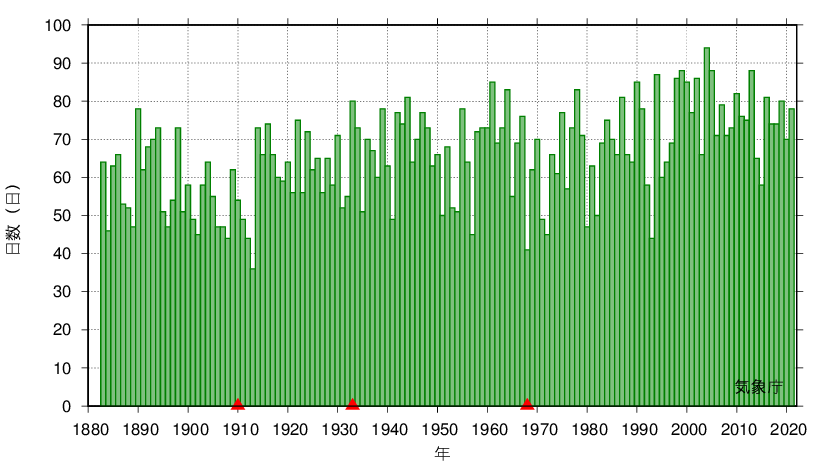
\includegraphics[width=\linewidth]{img/OSAKA_tmaxGE30.png}
      \subcaption{大阪 真夏日}
      \label{subfig1:temp_osaka}
    \end{minipage}\\
    \begin{minipage}[b]{\linewidth}
      \centering
      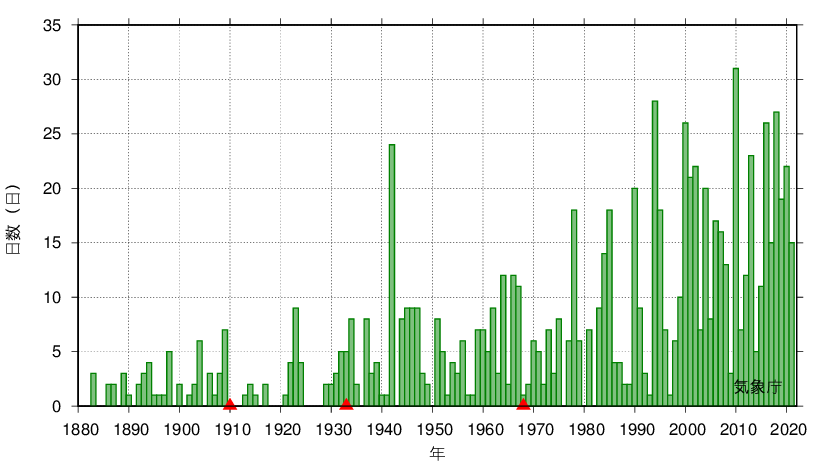
\includegraphics[width=\linewidth]{img/OSAKA_tmaxGE35.png}
      \subcaption{大阪 猛暑日}
      \label{subfig1:temp_osaka2}
    \end{minipage}
    \caption{真夏日および猛暑日の年間日数 1883-2021年\cite{temp_osaka3}}
    \label{fig1:temp_osaka}
\end{figure}
 

空調および冷凍分野において空気を冷やす原理として, "冷凍サイクル" が挙げられる. 
\figref{fig1:cycle}に示す通り, 冷凍サイクルは 「圧縮」「凝縮」「膨張」「蒸発」 
の4行程で構成されている. 冷凍サイクルにおいてモリエル線図(\figref{fig1:ph_r410}) 
は使用する冷媒の状態変化に伴う運転状況の変化, 装置能力, 装置動力などの計算に
よく使用される. 
上記に示した気温上昇に伴い, 今後は空調機の利用機会が増えると予想できる. 一般に
空調機には室内機と室外機に分類されており, 
冷房時において, 室外機は圧縮と凝縮, 室内機は蒸発と膨張の行程をそれぞれ担っている. 
室外機は高圧化した冷媒ガスを外気に熱を伝達することにより凝縮させ, 
室内機では, 膨張した冷媒液を室内の空気と熱交換させて冷媒の潜熱を利用して冷却する. 

\begin{figure}[hhtb]
  \centering
      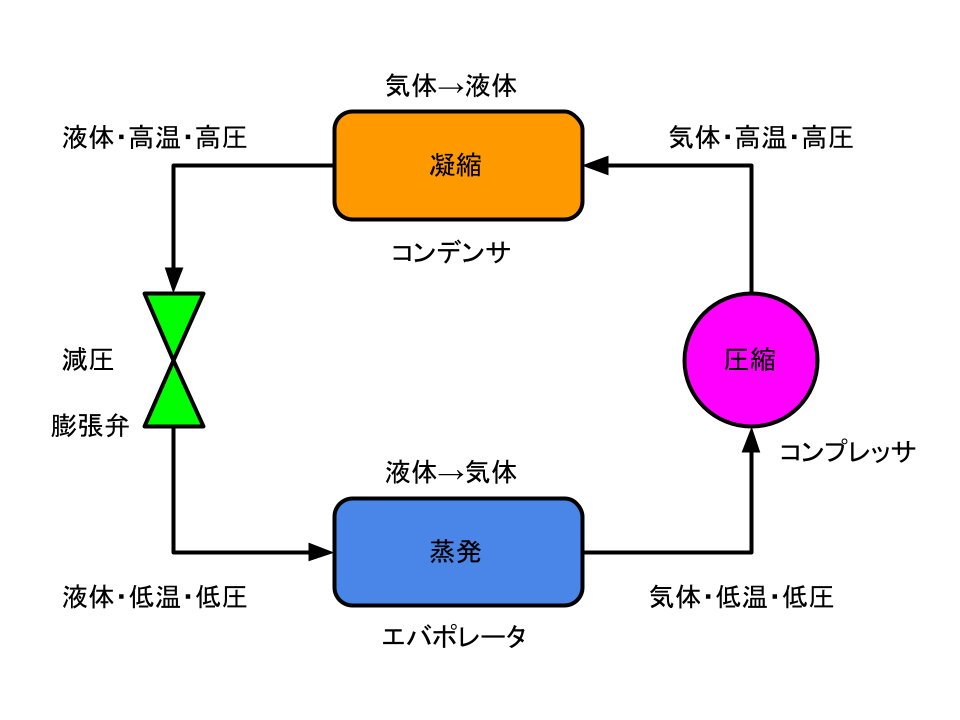
\includegraphics[width=0.8\linewidth]{img/cycle-2.png}
      \caption{冷凍サイクル}
      \label{fig1:cycle}
\end{figure}

\begin{figure}[hhtb]
    \centering
        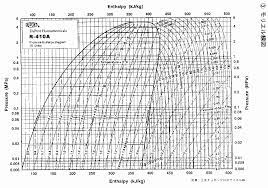
\includegraphics[width=\linewidth]{img/ph線図.jpg}
        \caption{モリエル線図(p-h 線図) 冷媒:R410}
        \label{fig1:ph_r410}
\end{figure}

ここで, 室外機吸い込み側空気, つまり外気温度が上昇すると, それに付随して凝縮温度
が高くなる. それにより冷却能力は小さくなり, 圧縮機駆動の駆動力が大きくなるため, 
成績係数が小さくなる. したがって, 同じ冷凍能力を出すためには消費電力が大きくなる.  
実際に外気温30℃, 相対湿度50\%の環境下で簡易的に10分おきにバケツにて散水をしながら
電力量を計測した. その対照実験の計測環境は\tableref{table:ex1}のとおりである. 

\begin{table}[hhtb]
  \caption{計測環境}
  \label{table:ex1}
  \centering
  \begin{tabular}{lcccc}
     & 外気温 & 湿度 & 設定温度 & 気候 \\
    \hline \hline
    実験1 & 34.3 & 48.0 & 27 & 晴れ  \\
    実験2 & 32.9 & 58.9 & 27 & 曇り \\
    \hline
  \end{tabular}
\end{table}

\figref{fig1:compare_watering}に示すように, 実験2 (散水あり) の電力量は実験1 (散水なし) のそれと
比較して小さくなっていることが分かる.

% 散水の有無の電力比較
\begin{figure*}[hhtb]
  \centering
      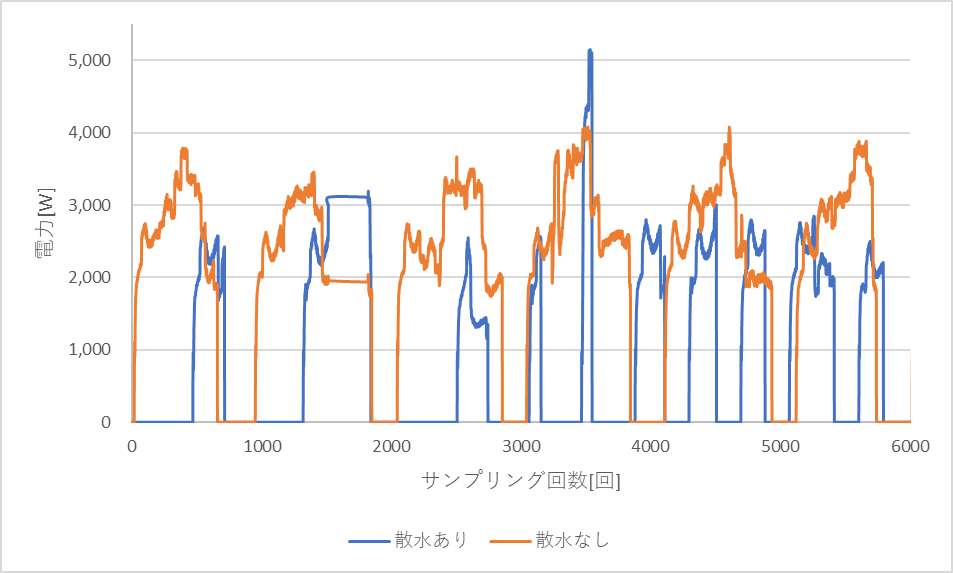
\includegraphics[width=\linewidth]{img/ex1.png}
      \caption{散水の有無による電力量の比較}
      \label{fig1:compare_watering}
\end{figure*}


% \begin{table*}[hhtb]
%   \caption{エアコン冷房時 電気代}
%   \label{table:aircon}
%   \centering
%   \begin{tabular}{lrrrr}
%     エアコン6畳タイプ & 最小消費電力 & 最大消費電力 & 期間消費電力量 & 1時間の電気代 \\
%      & [W] & [W] & [Wh] & [円] \\
%     \hline \hline
%     DAIKIN AN22YRS-W & 115 & 960 & 630 & 17.0 \\
%     Panasonic CU-X221D & 110 & 920 & 586 & 15.8 \\
%     SHARP AY-N22X & 130 & 810 & 578 & 15.6 \\
%     三菱電機 MSZ-ZW2221 & 105 & 850 & 594 & 16.0 \\
%     日立 RAC-X22L & 115 & 880 & 555 & 15.0 \\
%     \hline
%   \end{tabular}
% \end{table*}


\subsection{目的}\label{purpose}
\subsecref{background} より, 室外機において散水システムの導入が効果的であるという事が分かった. 
そこで本研究では, 散水システムの導入に伴い自作散水システムや市販の機器など様々な条件で比較検証を行い, 
電気代および水道代とのコストバランスを考慮しながら, 最適な散水システムを検討することを目的とする. 

\section{調査内容}\label{sec2}
本章では本研究で行った計測のための調査内容について説明する. 
本研究で調査対象とした室外機はビル用マルチエアコンである三菱社 
PUHY-EP335DMG9を採用した (\figref{subfig:condensing_unit}). 
室内機は本社2階の事務室に設置された天井吊り下げ式のユニットクーラーである三菱社 
○○○○である. 

\begin{figure}[hhtb]
  \centering
    \begin{minipage}[b]{0.45\linewidth}
      \centering
      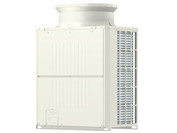
\includegraphics[width=\linewidth]{img/PUHY-EP335DMG9.jpg}
      \subcaption{PUHY-EP355DMG9}
      \label{subfig:condensing_unit}
    \end{minipage}
    \begin{minipage}[b]{0.45\linewidth}
      \centering
      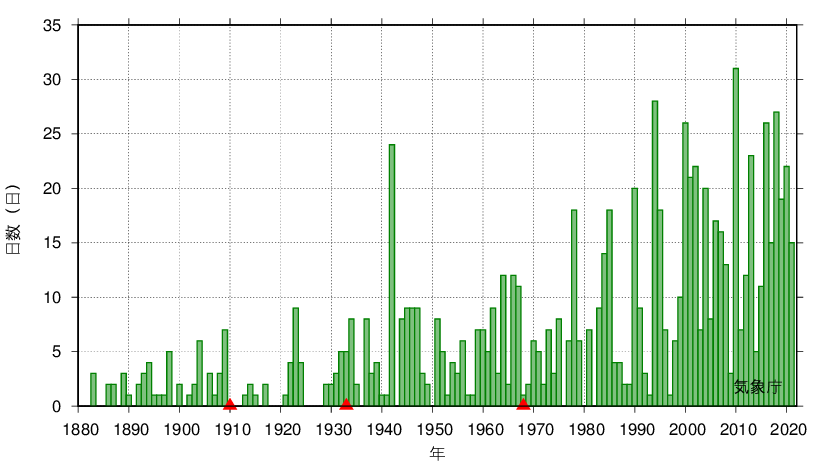
\includegraphics[width=\linewidth]{img/OSAKA_tmaxGE35.png}
      \subcaption{室内機挿入予定}
      \label{subfig:unit_cooler}
    \end{minipage}
  \caption{計測対象}
  \label{fig2:hard}
\end{figure}

\begin{table}[hhtb]
  \caption{機器仕様(冷房時)}
  \label{table:hard}
  \centering
  \begin{tabular}{lr}
    PUHY-EP355DMG9 & \\
    \hline \hline
    電源 & 3相 200V \\
    能力 & 33.5 kW \\
    消費電力 & 10.7 kW \\
    冷媒 & R410 \\
     & \\
    ○○○○ & \\
    \hline \hline
    電源 & 3相 200V \\
    能力 &  kW \\
    消費電力 &  kW \\
    \hline
  \end{tabular}
\end{table}


\subsection{自作散水システム}
本節では, 計測実験の比較対象として自作する散水システムの概要について説明する. 

\figref{fig2:watering_sys}に示す通り, 屋上にある蛇口からホースと塩化ビニル管を結合させて
室外機まで通し, 散水ノズルを用いて設置した. 

\begin{figure}[hhtb]
  \centering
    \begin{minipage}[b]{\linewidth}
      \centering
      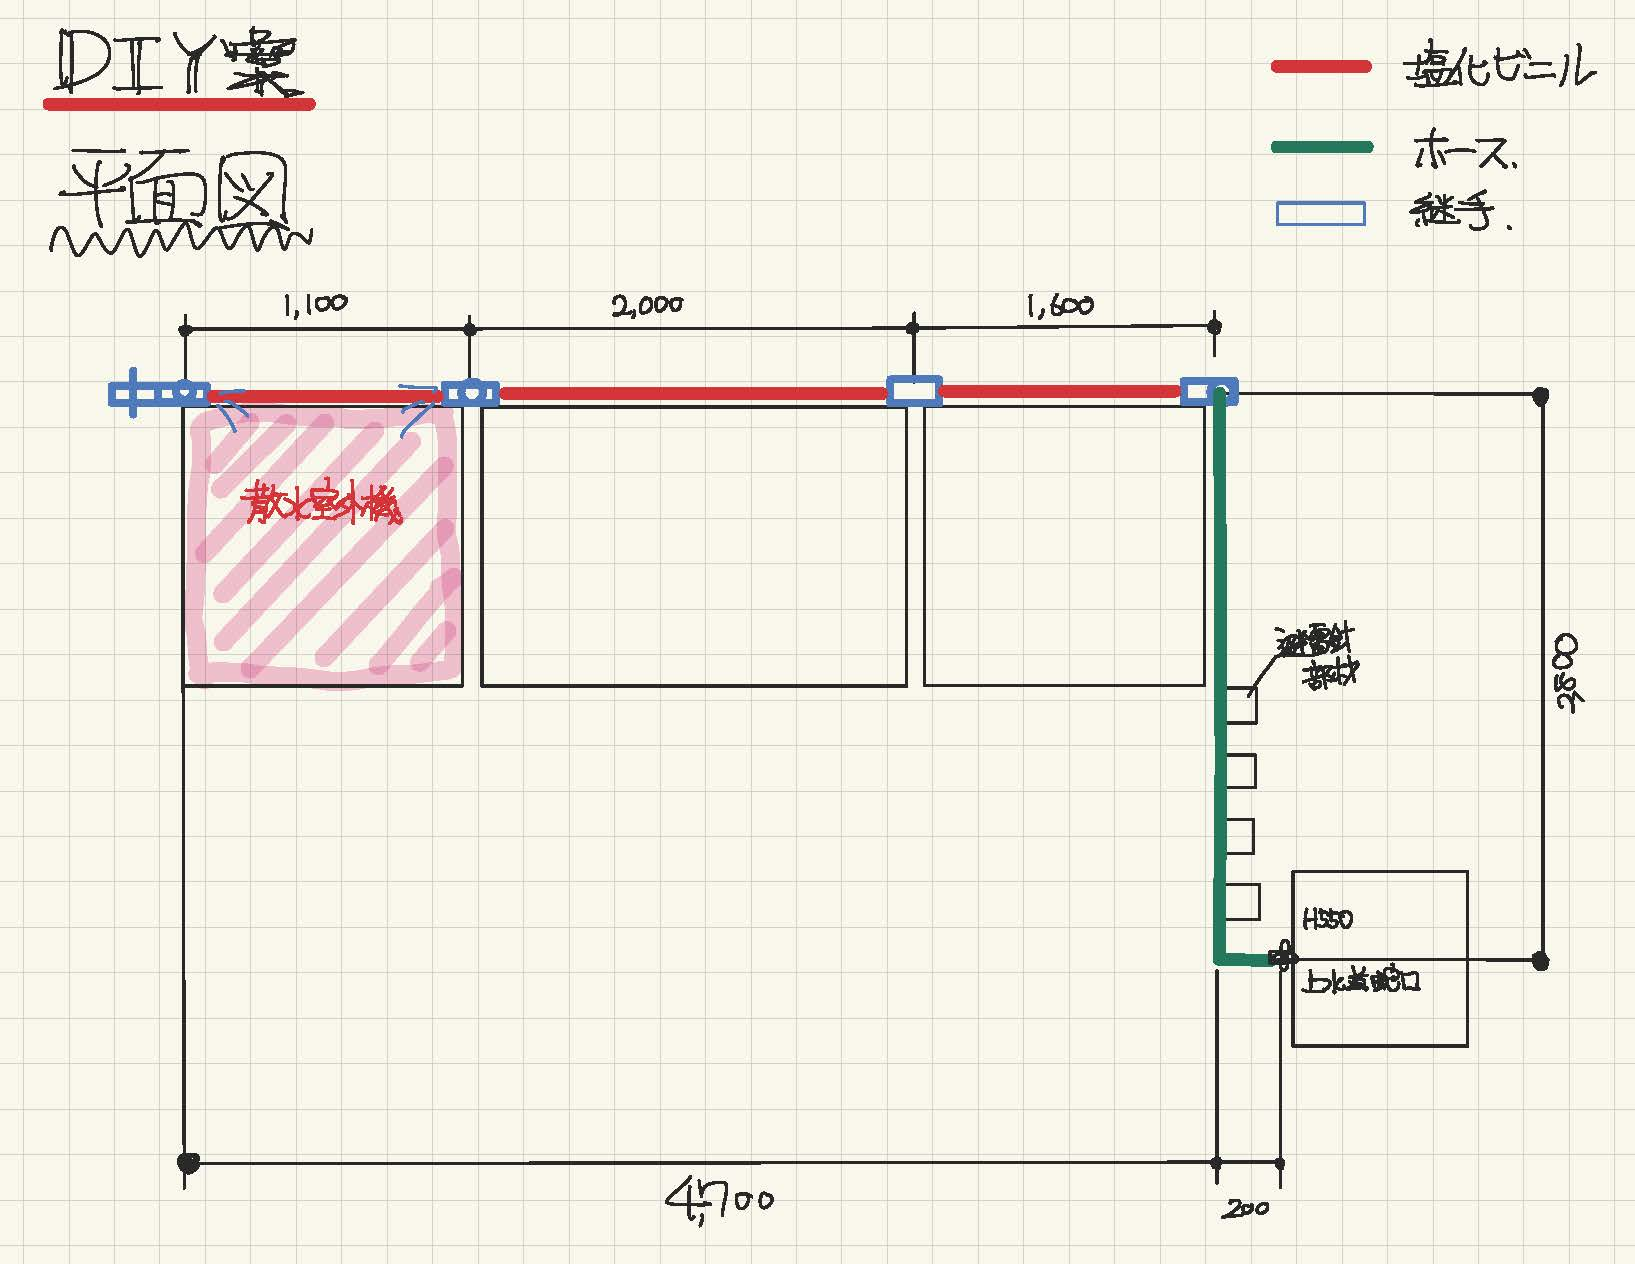
\includegraphics[width=\linewidth]{img/平面図.jpg}
      \subcaption{平面図}
      \label{subfig:平面図}
    \end{minipage}\\
    \begin{minipage}[b]{\linewidth}
      \centering
      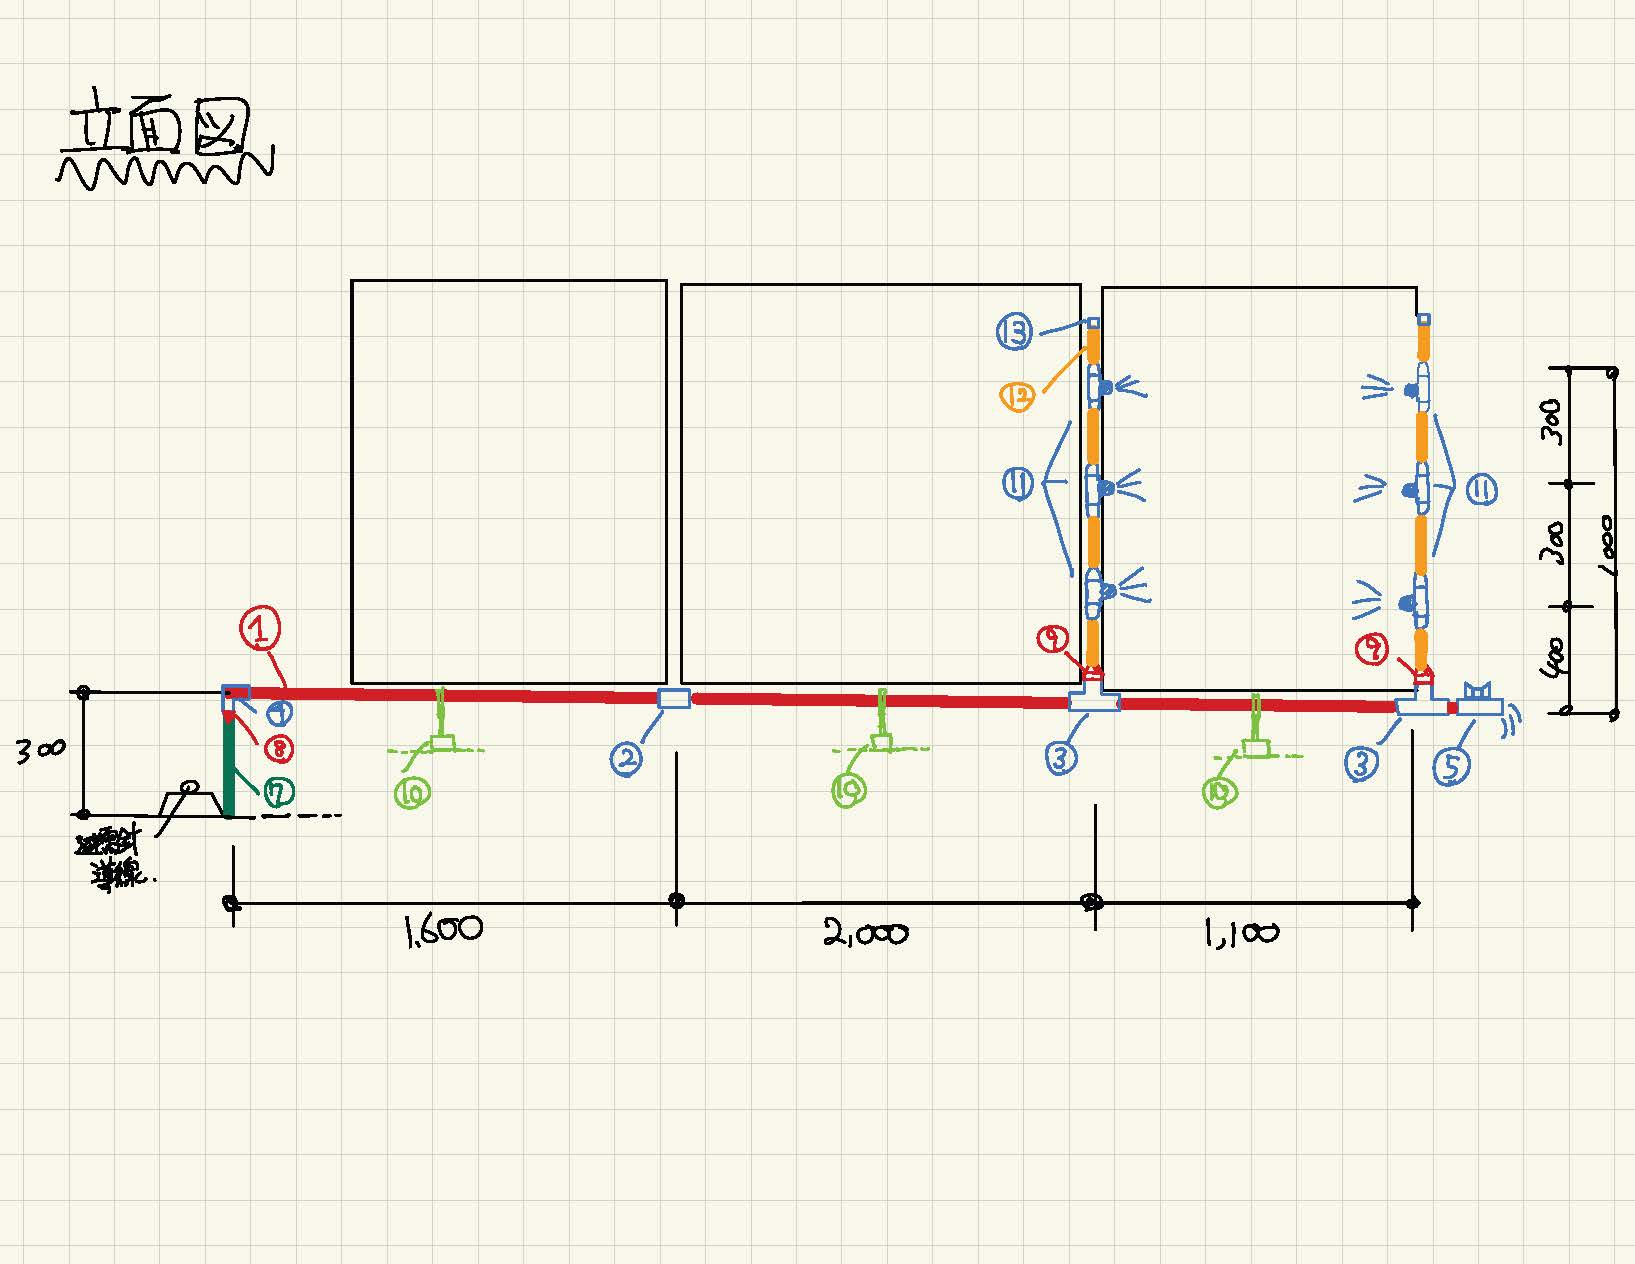
\includegraphics[width=\linewidth]{img/裏手立面図.jpg}
      \subcaption{裏手立面図}
      \label{subfig:裏手立面図}
    \end{minipage}
  \caption{散水システム設計図}
  \label{fig2:watering_sys}
\end{figure}

\subsection{計測}
計測したパラメータは以下の通りである. 

\begin{itemize}
  \item 外気環境(気温, 相対湿度, 風速)
  \item 凝縮器入口温度 (2箇所)
  \item 凝縮器出口温度 (2箇所)
  \item 電気系パラメータ (電流, 電圧, 電力量)
  \item 散水系パラメータ (水温, 散水流量)
\end{itemize}


\section{結果}\label{sec3}
計測環境は以下の4条件に分けて行った. 

\begin{description}
  \item[  Experiment1] 散水なし
  \item[  Experiment2] 散水あり (手動)
  \item[  EXperiment3] 散水あり (自作)
  \item[  EXperiment4] 散水あり (市販)
\end{description}

また, 各条件での計測結果は\tableref{table:ex}に示す通りである. 

\begin{table}[htb]
  \caption{計測環境}
  \label{table:ex}
  \centering
  \begin{tabular}{lrrrrr}
    実験 & 気温 & 湿度 & \small 比エンタルピー & \small 設定温度 & 気候 \\
     & [℃] & [\%] & [kJ/kg] & [℃] &  \\
    \hline \hline
    Ex1 & 34.3 & 48.0 & 76.5 & 27.0 & 晴れ  \\
    Ex2 & 32.9 & 58.9 & 80.9 & 27.0 & 曇り \\
    Ex3 &  &  &  & 27.0 & 晴れ \\
    Ex4 &  &  &  & 27.0 & 晴れ \\
    \hline
  \end{tabular}
\end{table}

各計測実験での電力量との推移は\figref{fig1:compare_watering}に示す. 

\section{考察}
従量電気料金を25円として見積もった際の各実験における電気代は\tableref{table:electric_bill}に示す. 

\begin{table}[htb]
  \caption{1時間あたりの電気料金}
  \label{table:electric_bill}
  \centering
  \begin{tabular}{lrr}
    実験 & 消費電力 & 電気代[円] \\
    \hline \hline
    Ex1 &  & 34 \\
    Ex2 &  & 32 \\
    Ex3 &  &  \\
    Ex4 &  &  \\
    \hline
  \end{tabular}
\end{table}

\section{結論}
本章では計測結果および考察を総括した結論を示す. 

%参考文献
\begin{thebibliography}{99}
\bibitem{temp_osaka}
国土交通省, 気象庁, 大阪府 日最高気温の月平均値, 
\url{https://www.data.jma.go.jp/obd/stats/etrn/view/monthly_s3.php?prec_no=62&block_no=47772&year=&month=&day=&view=a2}\vspace{2mm}

\bibitem{temp_osaka2}
George's Web Sites, 大阪府-大阪市の気温に関する統計情報, 
\url{http://www.tvg.ne.jp/george/weather/gw_stat_temp.html?city=oosaka}\vspace{2mm}

\bibitem{temp_osaka3}
A-PLAT 気候変動適応プラットフォーム, 気候変動の観測・予測データ, 大阪府観測データ, 
\url{https://adaptation-platform.nies.go.jp/map/Osaka/index_past.html}\vspace{2mm}
\end{thebibliography}
%
%
%
\end{document}